\documentclass[UTF8]{ctexart}

\usepackage{graphicx}
\usepackage{geometry}
\usepackage{booktabs}
\usepackage{longtable}
\usepackage{float}

\geometry{a4paper, scale=0.8}

\title{社交网络欺诈检测项目报告}
\author{}
\date{\today}

\begin{document}

\maketitle

\tableofcontents


\section{项目引言}

\subsection{项目背景}

随着社交网络的迅猛发展，它们已成为人们日常生活不可或缺的一部分。然而，这种普及性也催生了大量的恶意行为，如虚假账户、网络钓鱼、垃圾信息传播和身份盗用等。这些欺诈行为不仅损害了用户体验，还可能导致严重的用户经济损失和平台声誉受损。因此，开发高效、准确的欺诈检测系统对于维护社交网络生态的健康与安全至关重要。

\subsection{项目目标}

本项目旨在利用机器学习和社交网络分析技术，构建一个能够自动识别社交网络中欺诈用户的模型。主要目标包括：

\begin{itemize}
    \item \textbf{数据探索与预处理}: 对真实的社交网络数据集进行深入的探索性数据分析（EDA），理解用户行为特征和网络结构。
    \item \textbf{模型构建与训练}: 基于用户属性和行为数据，训练和评估多种机器学习分类模型（如逻辑回归、随机森林），以区分正常用户和欺诈用户。
    \item \textbf{社交网络分析}: 构建用户间的社交关系图，分析其网络拓扑特性，并探索如何利用网络结构信息来增强欺诈检测的效果。
    \item \textbf{性能评估与优化}: 采用合适的评估指标（如精确率、召回率、F1分数、ROC-AUC），系统地评估模型性能，并针对数据不平衡问题进行优化。
\end{itemize}

\subsection{数据集介绍}

本项目使用了公开的社交网络欺诈检测数据集 Fakhraei et al. (2015)，该数据集包含两部分：
\begin{itemize}
    \item `usersdata.csv`: 用户的个人资料和行为特征。
    \item `relations.csv`: 用户之间的关注关系。
\end{itemize}

标签信息将从用户特征中提取，用于监督学习。

\subsection{项目意义}

通过本项目的研究与实践，我们期望能够：
\begin{itemize}
    \item 为社交平台提供一种有效的欺诈用户检测方案。
    \item 深入理解欺诈用户在行为和网络结构上的特征。
    \item 为后续更复杂的混合模型（结合内容、行为和网络信息）研究提供基础。
\end{itemize}

\section{数据探索与分析}

\subsection{用户特征分析}

我们首先对 `usersdata.csv` 数据集进行了探索性分析，以理解用户特征的分布情况。该数据集包含了用户的多种属性，如账户年龄、粉丝数、关注数、状态更新频率等。

\begin{figure}[H]
    \centering
    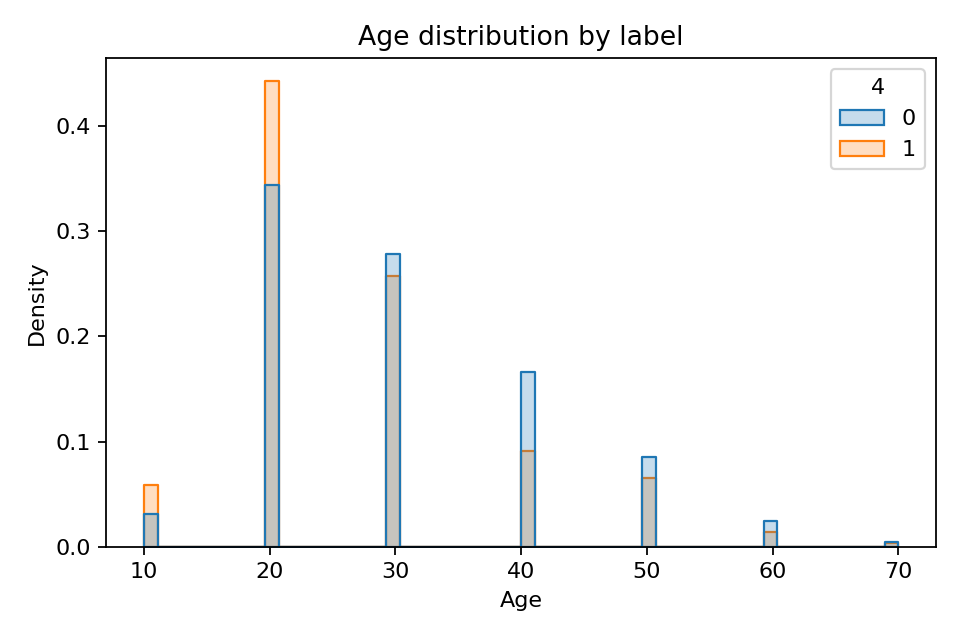
\includegraphics[width=0.8\textwidth]{output/fakhraei/users_age_hist.png}
    \caption{用户账户年龄分布直方图}
    \label{fig:user_age_hist}
\end{figure}

为了更好地理解不同特征之间的关系，我们绘制了特征的散点图矩阵。

\begin{figure}[H]
    \centering
    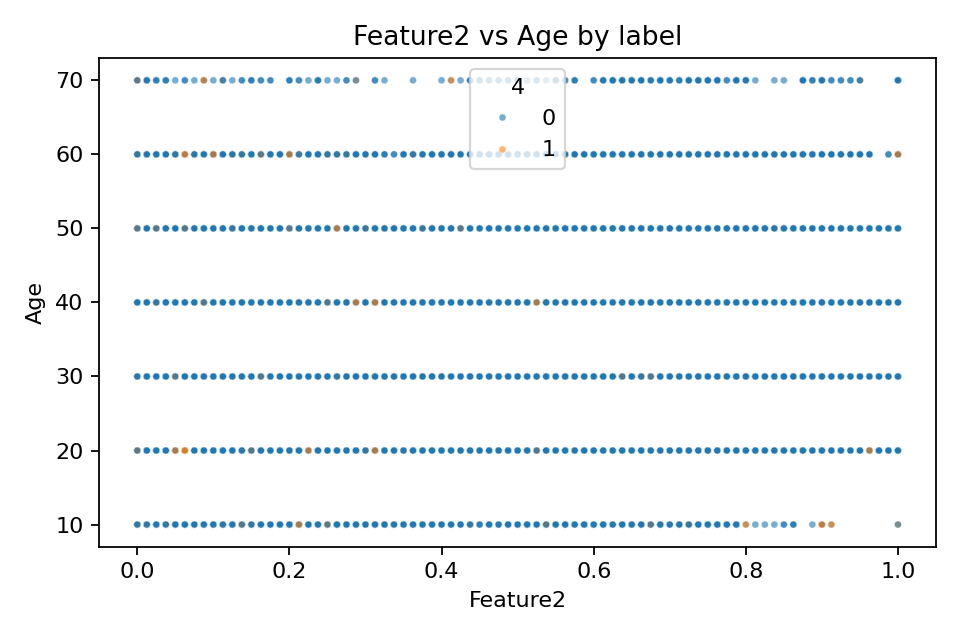
\includegraphics[width=\textwidth]{output/fakhraei/users_scatter.png}
    \caption{用户特征散点图矩阵}
    \label{fig:user_scatter}
\end{figure}

\subsection{数据降维与可视化}

为了在二维空间中可视化高维的用户特征数据，我们采用了 t-SNE (t-Distributed Stochastic Neighbor Embedding) 降维技术。下图清晰地展示了正常用户和欺诈用户在特征空间中的分布情况，欺诈用户（红色）在某些区域呈现出明显的聚集性。

\begin{figure}[H]
    \centering
    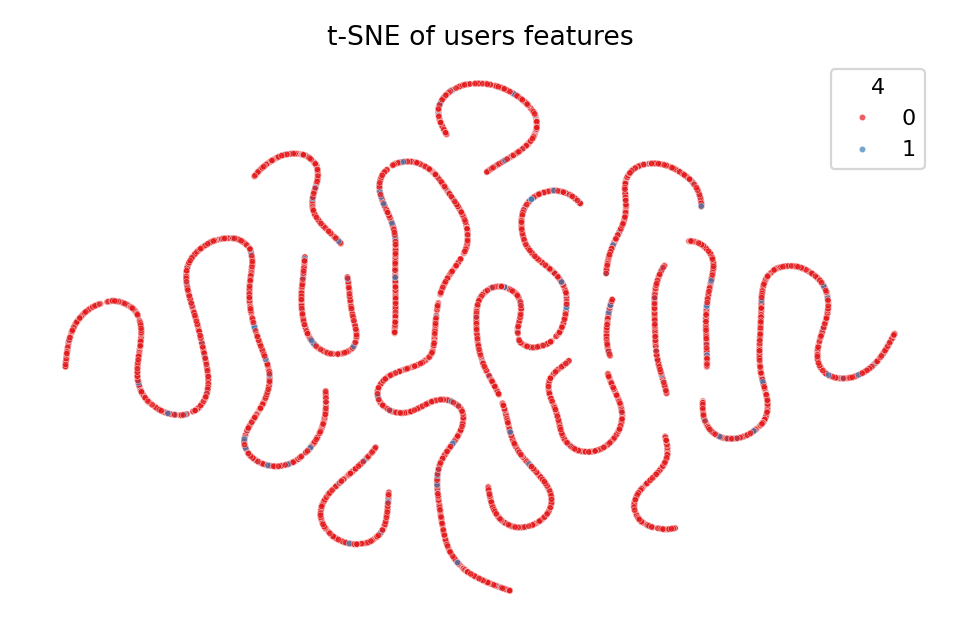
\includegraphics[width=0.8\textwidth]{output/fakhraei/users_tsne.png}
    \caption{用户特征的t-SNE降维可视化 (欺诈用户以红色标出)}
    \label{fig:user_tsne}
\end{figure}

\section{研究方法}

\subsection{数据预处理与特征工程}

在模型训练之前，我们对数据进行了系统的预处理，步骤如下：
\begin{enumerate}
    \item \textbf{特征提取}: 从原始数据中筛选出所有数值型特征用于建模。
    \item \textbf{缺失值处理}: 将数据集中的无穷大或缺失值（NaN）统一替换为0.0。
    \item \textbf{数据标准化}: 采用 `StandardScaler` 对特征进行标准化处理，消除不同特征之间的量纲差异，使模型能够更快、更稳定地收敛。
\end{enumerate}

\subsection{数据集划分}

为了保证模型评估的公正性和可靠性，我们将数据集划分为训练集、验证集和测试集。考虑到欺诈用户在数据集中占比较少（数据不平衡），我们采用\textbf{分层抽样}（Stratified Sampling）策略进行划分：
\begin{itemize}
    \item \textbf{训练集 (Training Set)}: 60% 的数据，用于训练模型。
    \item \textbf{验证集 (Validation Set)}: 20% 的数据，用于调整模型超参数（如决策阈值）。
    \item \textbf{测试集 (Test Set)}: 20% 的数据，用于最终评估模型的泛化能力。
\end{itemize}

这种划分方式确保了在训练、验证和测试三个集合中，欺诈用户和正常用户的比例与原始数据集保持一致。

\subsection{模型选择}

我们选择了两种具有代表性的分类模型进行欺诈检测：
\begin{enumerate}
    \item \textbf{逻辑回归 (Logistic Regression)}: 作为一个强大且解释性强的基准模型，它能提供一个基本的性能参考。
    \item \textbf{随机森林 (Random Forest)}: 作为一种集成学习模型，它通常具有更高的准确性和鲁棒性，并且能够评估特征的重要性。
\end{enumerate}

\subsection{不平衡数据处理}

欺诈检测任务通常面临严重的数据不平衡问题，即正常用户数量远超欺诈用户。为解决此问题，我们采取了以下策略：
\begin{itemize}
    \item \textbf{类别权重调整}: 在模型训练时，我们设置 \texttt{class\_weight='balanced'} 参数。这使得模型在训练时对少数类（欺诈用户）的样本给予更高的权重，从而减轻多数类对损失函数的主导影响。
    \item \textbf{决策阈值优化}: 分类模型的默认决策阈值为0.5，但这在不平衡数据上通常不是最优的。我们利用验证集来寻找一个最优的决策阈值，该阈值能够在验证集上最大化F1分数。然后，我们将此最优阈值应用于测试集，以获得更符合实际业务需求的预测结果。
\end{itemize}

\subsection{评估指标}

为了全面评估模型在不平衡数据上的性能，我们采用了多种评估指标：
\begin{itemize}
    \item \textbf{精确率 (Precision)、召回率 (Recall)、F1分数 (F1-Score)}: 核心的分类任务评估指标。
    \item \textbf{宏平均指标 (Macro-Average Precision/Recall/F1)}: 对每个类别的指标进行平均，平等对待每个类别，是评估不平衡数据分类性能的关键指标。
    \item \textbf{ROC-AUC (Area Under the ROC Curve)}: 衡量模型在所有可能阈值下的整体排序能力。
    \item \textbf{PR-AUC (Area Under the Precision-Recall Curve)}: 在不平衡数据集上，PR曲线比ROC曲线能更灵敏地反映模型性能的变化。
\end{itemize}

\section{模型性能评估}

本章将详细介绍和分析逻辑回归与随机森林模型在欺诈用户检测任务上的性能表现。

\subsection{模型性能总览}

我们将各模型在测试集上的核心性能指标进行了汇总，如下表所示。随机森林在宏平均F1分数（Macro-F1）上表现最佳，说明其在不平衡数据上的综合性能更优。

\begin{table}[H]
    \centering
    \caption{模型核心性能指标对比}
    \label{tab:model_performance}
    \begin{tabular}{lcccc}
        \toprule
        模型 & Macro F1-Score & ROC-AUC & PR-AUC & 备注 \\
        \midrule
        逻辑回归 & 0.463 & \textbf{0.761} & \textbf{0.258} & 基准模型 \\
        随机森林 (默认阈值) & \textbf{0.601} & 0.708 & 0.187 & 默认决策阈值 0.5 \\
        随机森林 (优化阈值) & - & 0.708 & 0.187 & 优化后阈值为 0.6 \\
        \bottomrule
    \end{tabular}
\end{table}

\subsection{ROC 与 PR 曲线分析}

ROC曲线和PR曲线能够直观地展示模型在不同决策阈值下的性能表现。

\begin{figure}[H]
    \centering
    \begin{minipage}{0.48\textwidth}
        \centering
        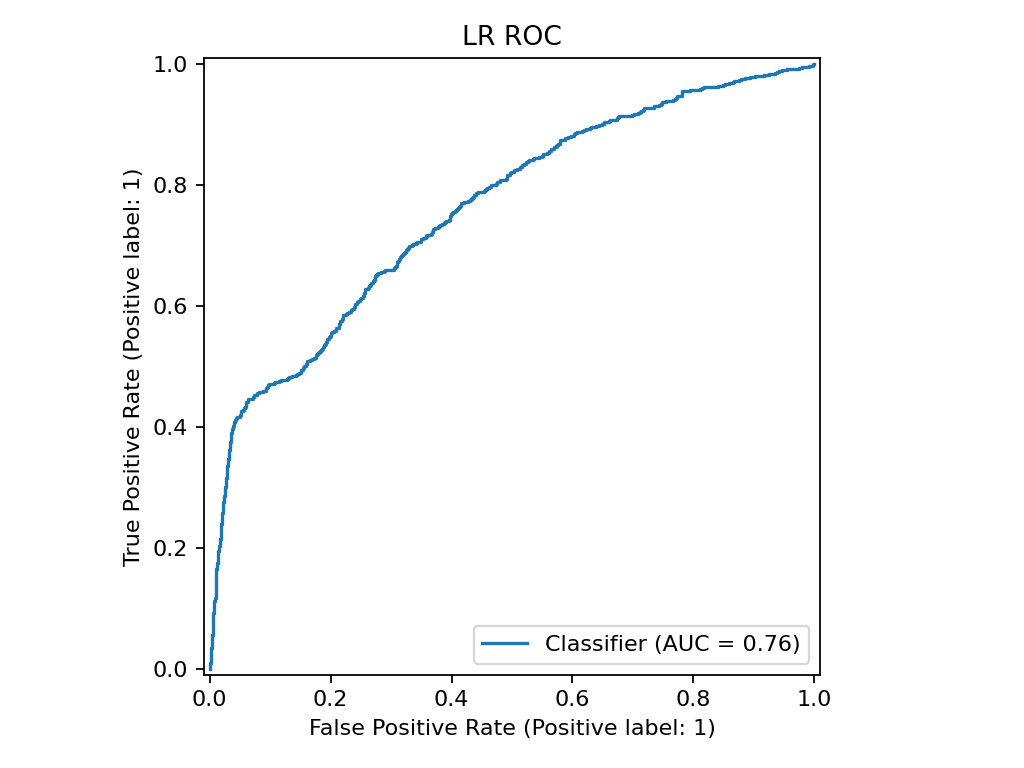
\includegraphics[width=\textwidth]{output/fakhraei/lr_roc.png}
        \caption{逻辑回归ROC曲线}
    \end{minipage}
    \hfill
    \begin{minipage}{0.48\textwidth}
        \centering
        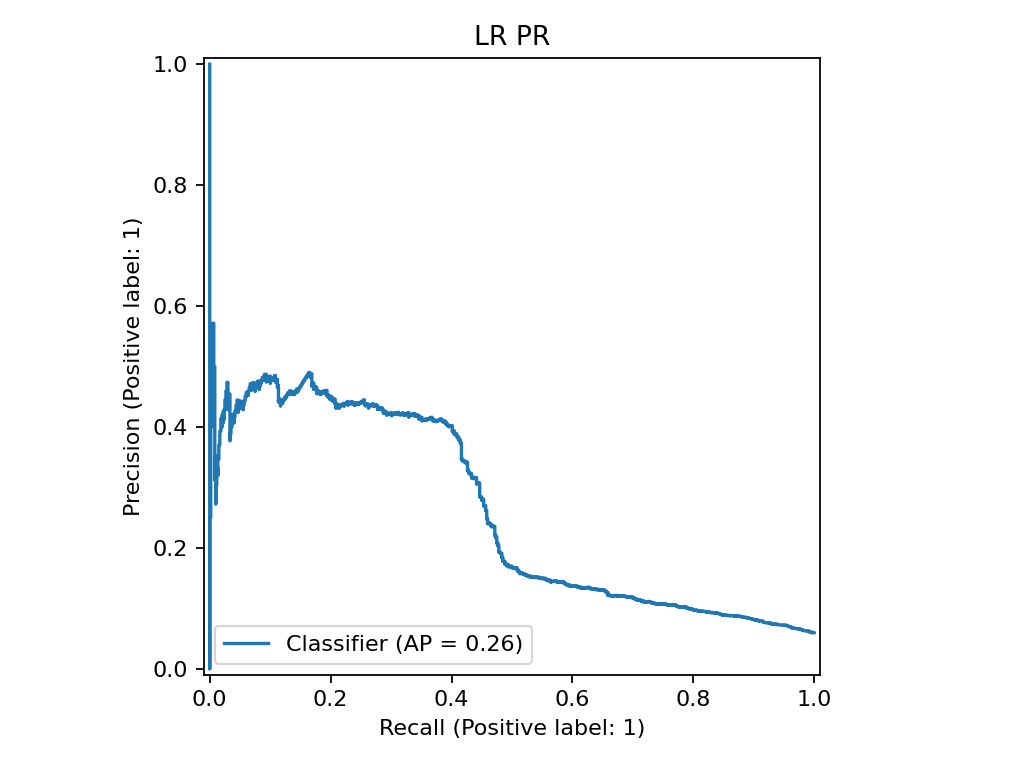
\includegraphics[width=\textwidth]{output/fakhraei/lr_pr.png}
        \caption{逻辑回归PR曲线}
    \end{minipage}
    \label{fig:lr_curves}
\end{figure}

\begin{figure}[H]
    \centering
    \begin{minipage}{0.48\textwidth}
        \centering
        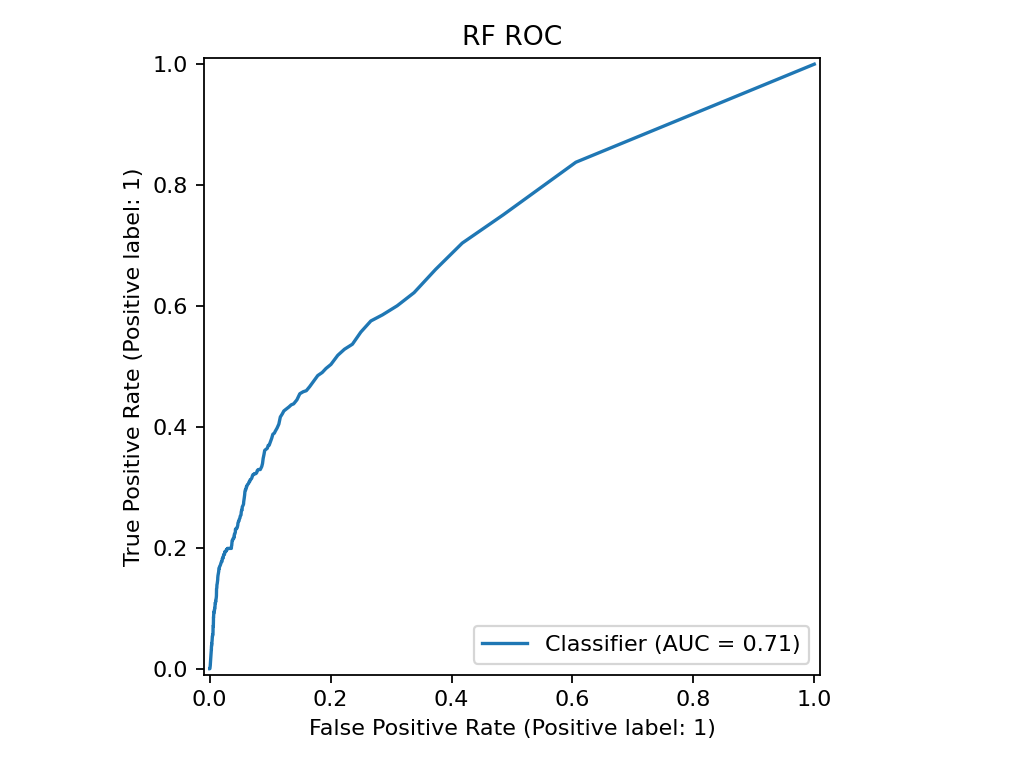
\includegraphics[width=\textwidth]{output/fakhraei/rf_roc.png}
        \caption{随机森林ROC曲线}
    \end{minipage}
    \hfill
    \begin{minipage}{0.48\textwidth}
        \centering
        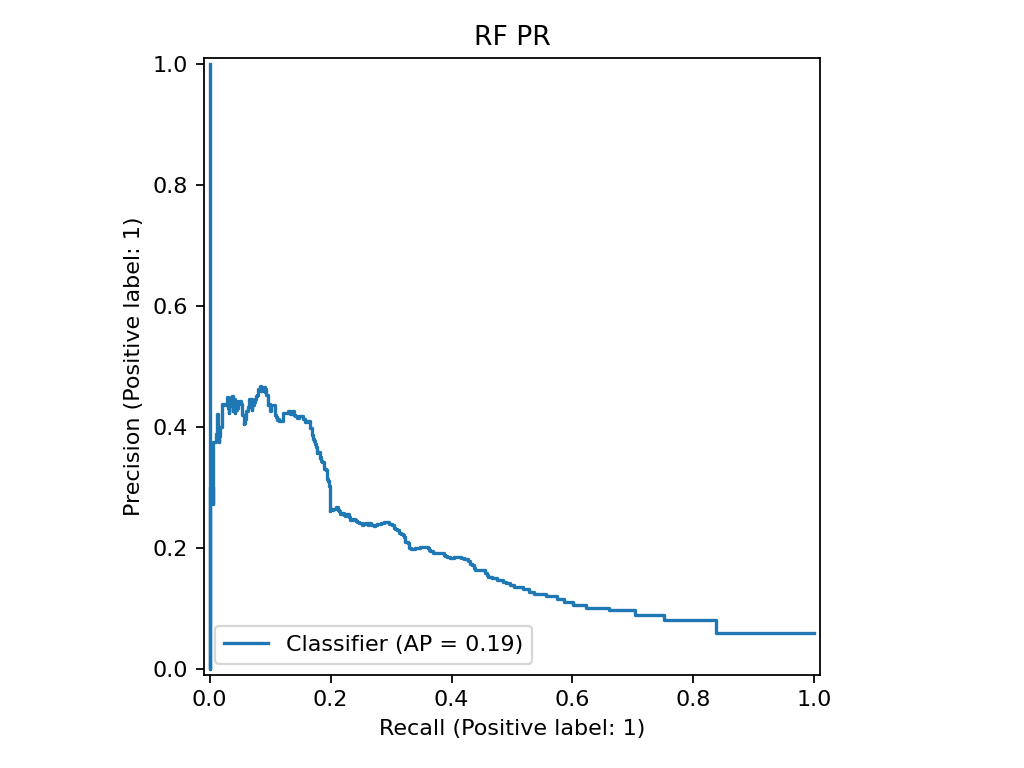
\includegraphics[width=\textwidth]{output/fakhraei/rf_pr.png}
        \caption{随机森林PR曲线}
    \end{minipage}
    \label{fig:rf_curves}
\end{figure}

从ROC曲线来看，逻辑回归（AUC=0.761）的排序能力略优于随机森林（AUC=0.708）。然而，在欺诈用户占比较低的不平衡场景下，PR曲线更有参考价值。逻辑回归的PR-AUC（0.258）显著高于随机森林（0.187），表明在召回率提升的过程中，逻辑回归能保持相对更高的精确率。

\subsection{混淆矩阵分析}

混淆矩阵清晰地展示了模型对正负样本的预测情况。我们重点分析性能更优的随机森林模型。

\begin{figure}[H]
    \centering
    \begin{minipage}{0.48\textwidth}
        \centering
        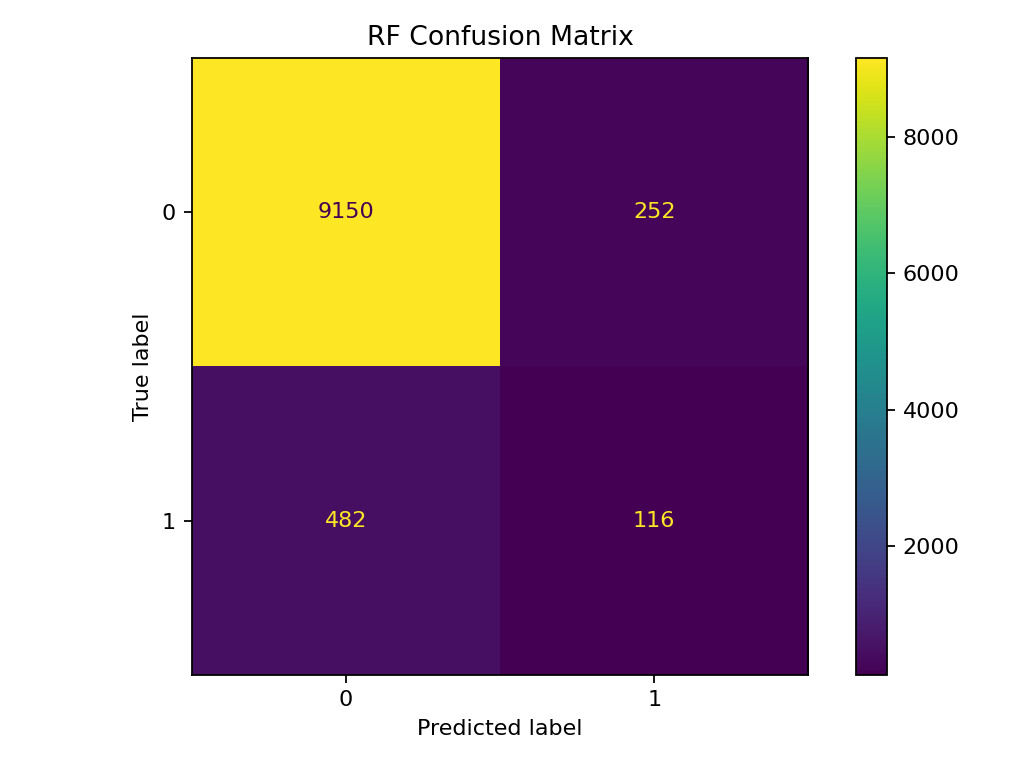
\includegraphics[width=\textwidth]{output/fakhraei/rf_cm.png}
        \caption{随机森林默认阈值混淆矩阵}
    \end{minipage}
    \hfill
    \begin{minipage}{0.48\textwidth}
        \centering
        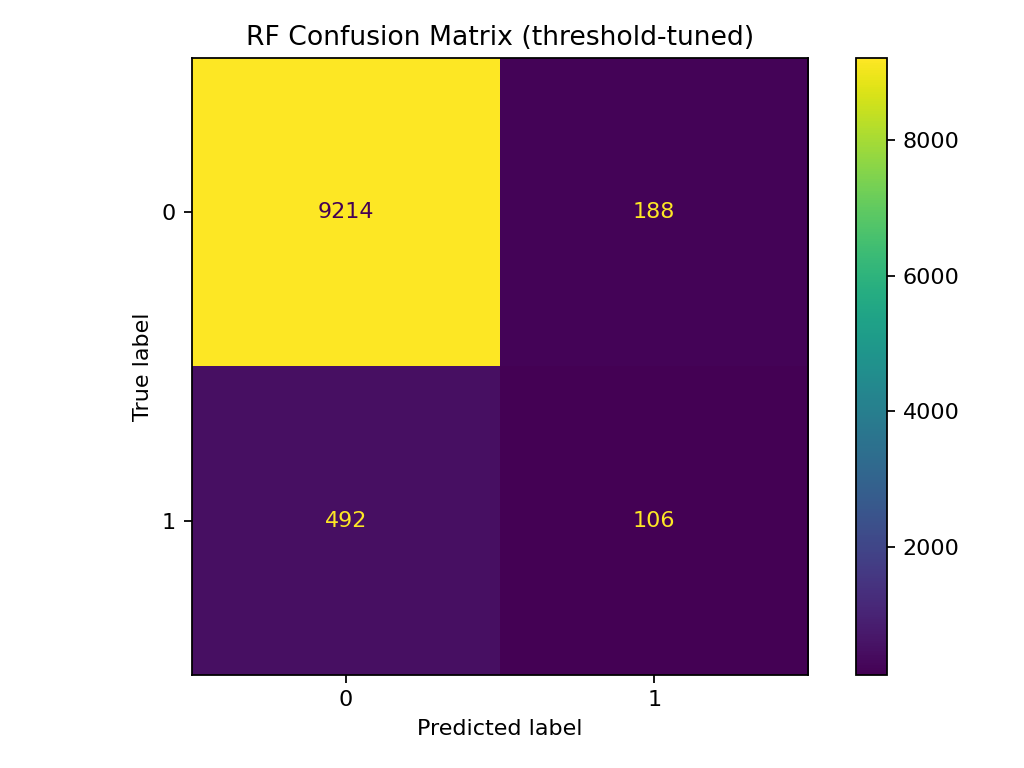
\includegraphics[width=\textwidth]{output/fakhraei/rf_cm_tuned.png}
        \caption{随机森林优化阈值混淆矩阵}
    \end{minipage}
    \label{fig:rf_cm}
\end{figure}

通过对比可以发现，默认阈值（0.5）下，模型倾向于将更多样本预测为正常用户，导致对欺诈用户的召回率较低。在验证集上优化阈值后（调整为0.6），虽然召回的欺诈用户数量略有下降，但精确率得到了提升，这在某些需要控制误报率的业务场景下可能更有价值。

\subsection{特征重要性分析}

随机森林模型能够评估各个特征对于分类决策的贡献度。下图展示了最重要的几个特征。

\begin{figure}[H]
    \centering
    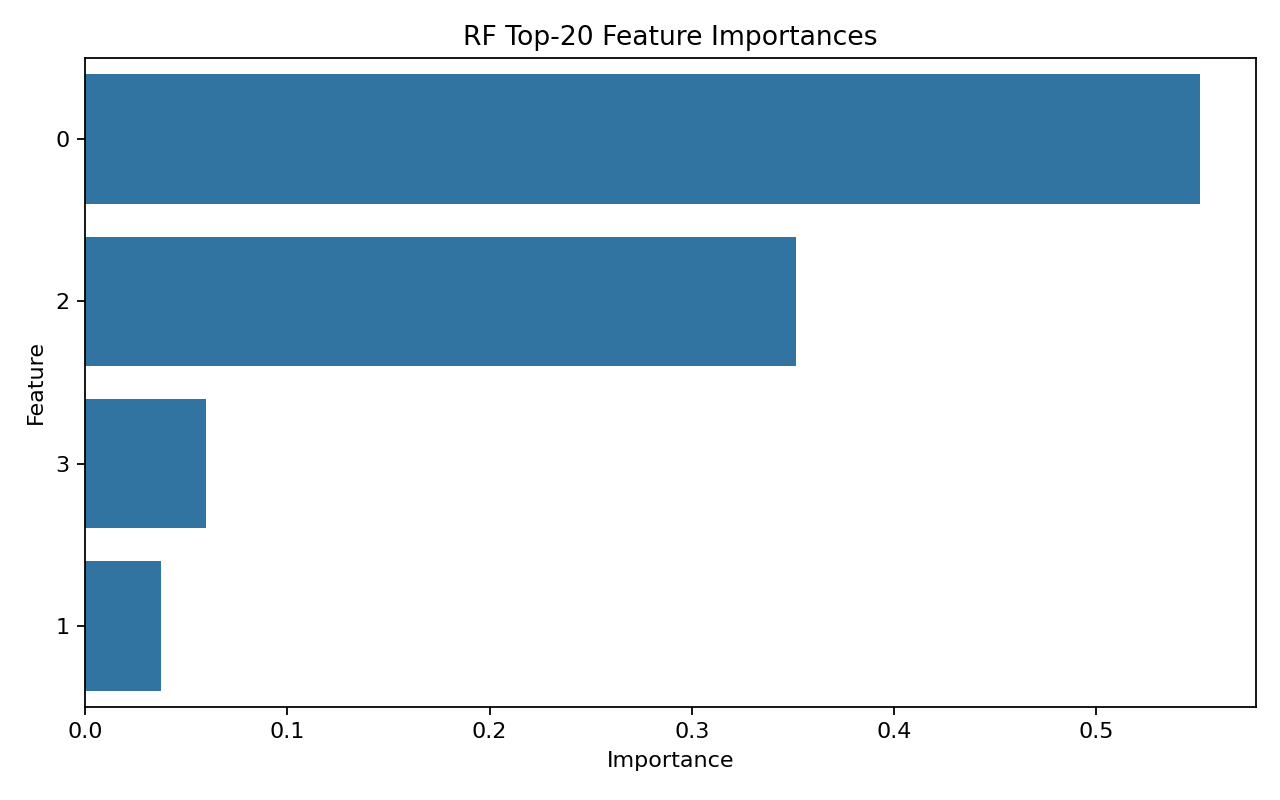
\includegraphics[width=0.8\textwidth]{output/fakhraei/rf_importance.png}
    \caption{随机森林模型的特征重要性排序}
    \label{fig:rf_importance}
\end{figure}

从图中可以看出，特征`3`和`2`是模型进行决策时最重要的依据，这为我们理解欺诈用户的行为模式提供了重要线索。

\section{社交网络分析}

除了基于用户属性的分类模型，我们还对用户之间的关注关系进行了网络分析，以挖掘潜在的结构化信息。

\subsection{网络构建与统计特性}

我们基于 `relations.csv` 文件构建了一个有向图，其中节点代表用户，边代表关注关系。由于原始图规模巨大，我们加载了前10万条边进行分析。网络的基本统计特性如下：

\begin{itemize}
    \item \textbf{节点数}: 161,742
    \item \textbf{边数}: 100,000
    \item \textbf{平均度}: 1.237
    \item \textbf{最大度}: 542
\end{itemize}

这些数据显示，该网络是一个高度稀疏的网络，大部分节点的连接数都很少。

\subsection{网络可视化与核心结构}

为了直观地展示网络结构，我们提取了度数最高的1000个节点构成的核心子图进行可视化。

\begin{figure}[H]
    \centering
    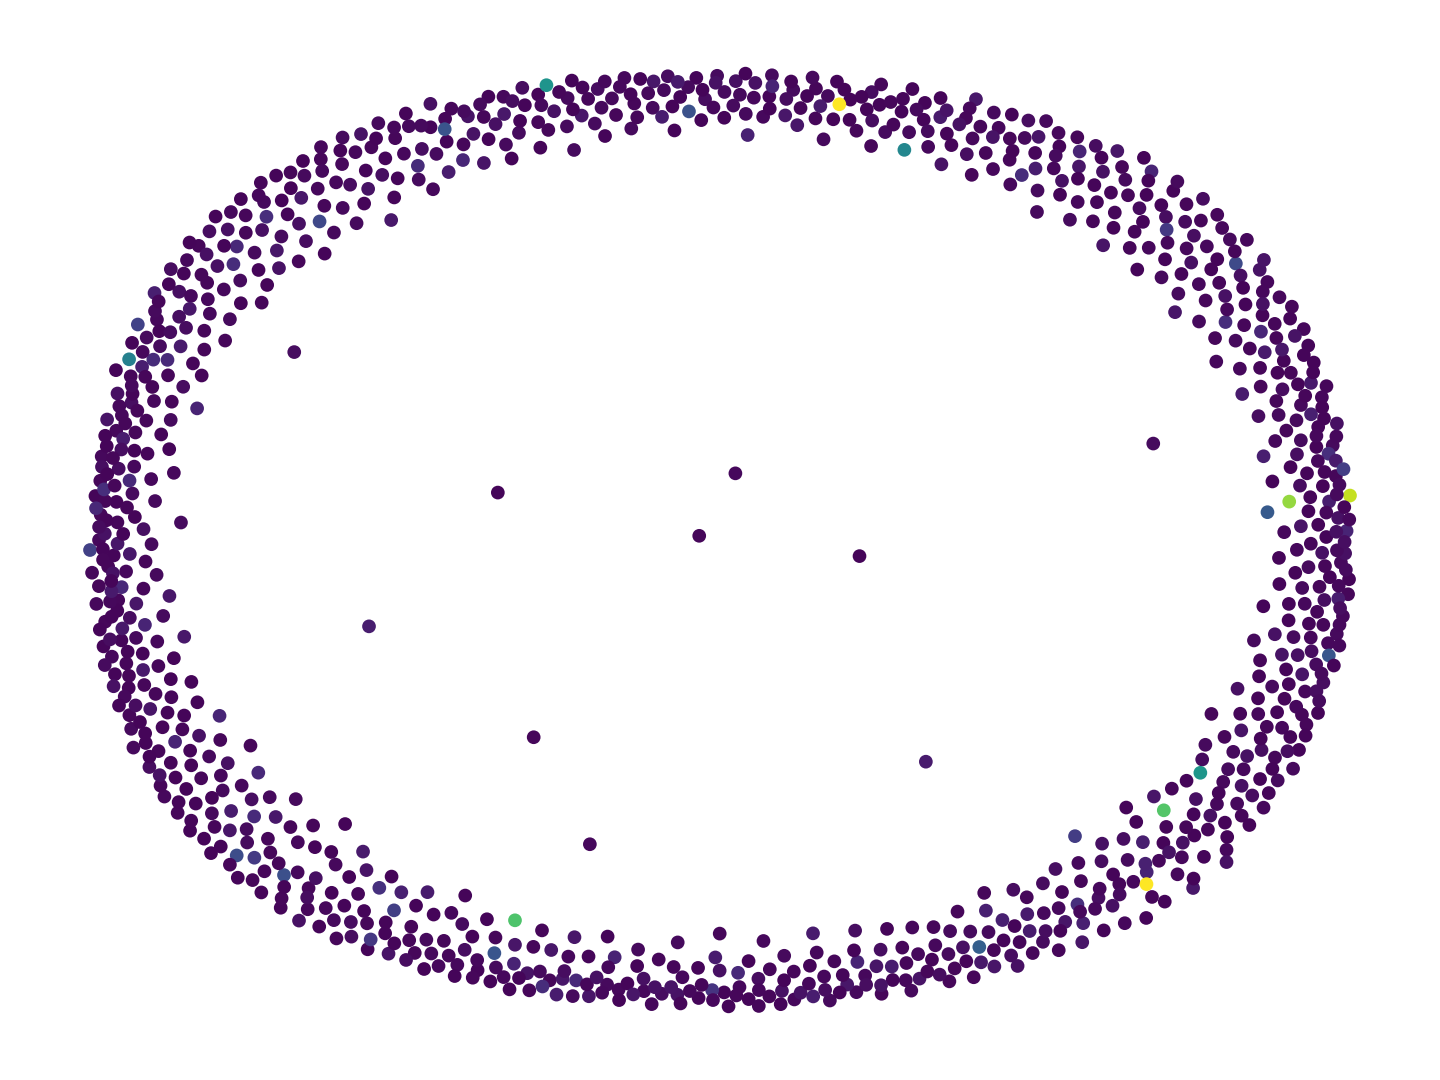
\includegraphics[width=0.8\textwidth]{output/fakhraei/social_graph.png}
    \caption{社交网络核心子图可视化}
    \label{fig:social_graph}
\end{figure}

从图中可以看到，网络中存在一些高度连接的“中心”节点（Hubs），这些节点连接了大量的其他用户，形成了网络的骨架。

\subsection{度分布分析}

度分布是衡量网络结构特性的重要指标。下图展示了网络中所有节点的度分布情况。

\begin{figure}[H]
    \centering
    \begin{minipage}{0.48\textwidth}
        \centering
        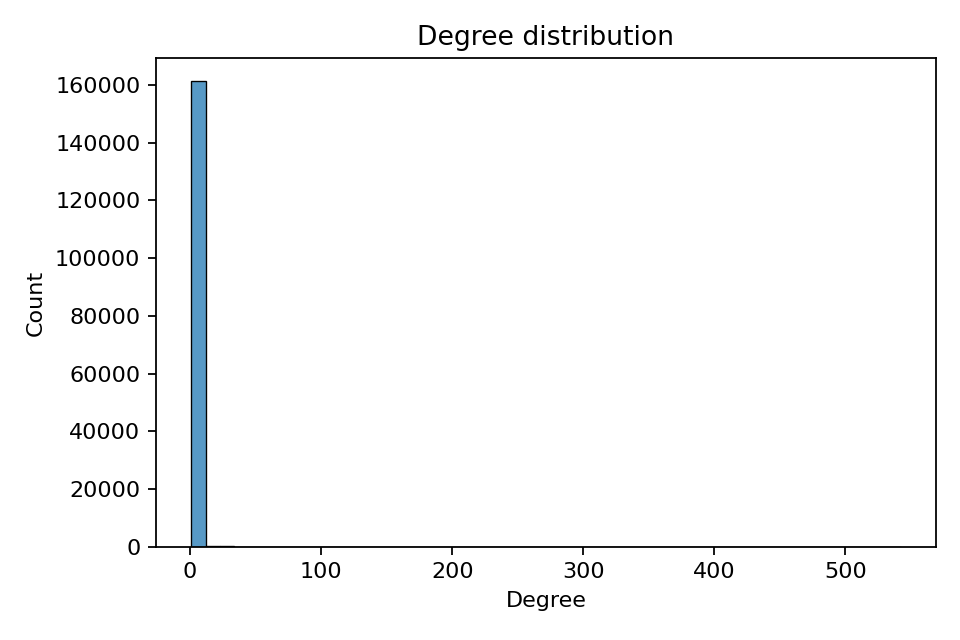
\includegraphics[width=\textwidth]{output/fakhraei/degree_hist.png}
        \caption{节点度分布直方图}
    \end{minipage}
    \hfill
    \begin{minipage}{0.48\textwidth}
        \centering
        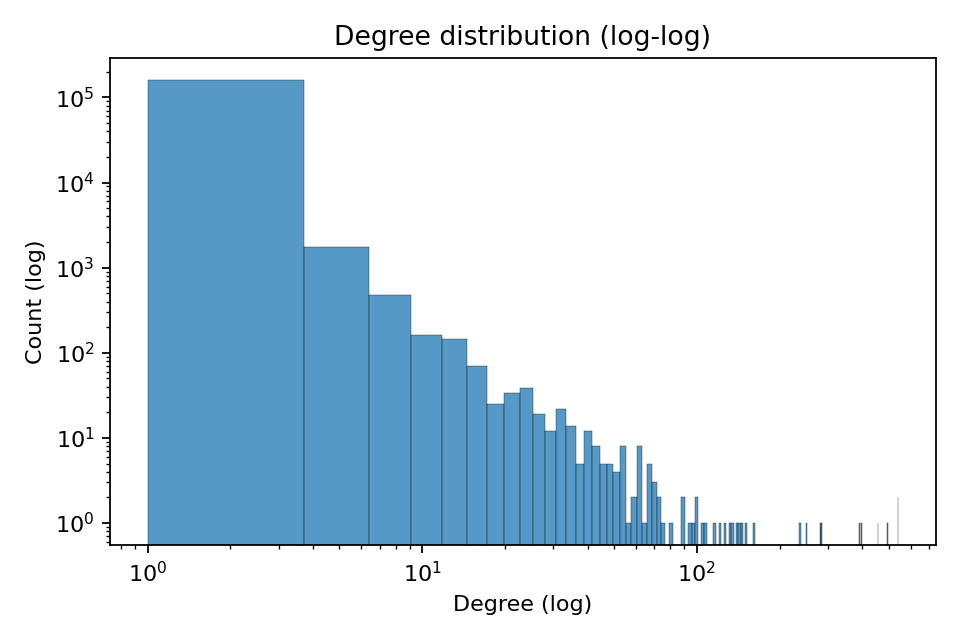
\includegraphics[width=\textwidth]{output/fakhraei/degree_loglog.png}
        \caption{节点度分布对数-对数图}
    \end{minipage}
    \label{fig:degree_dist}
\end{figure}

左图显示，绝大多数节点的度都非常低（小于10），符合稀疏网络的特征。而右侧的对数-对数坐标图显示，度分布近似于一条直线，这表明网络具有\textbf{无标度（Scale-Free）特性}或\textbf{重尾分布}。这种“富者愈富”的现象是真实世界社交网络的典型特征，即少数核心用户拥有极高的连接度，而大部分边缘用户只有少量连接。这种结构对于信息传播和网络鲁棒性有重要影响，也可能与欺诈行为的传播模式有关。

\section{结论与展望}

\subsection{项目总结}

本项目成功地应用了机器学习和社交网络分析技术，对社交网络中的欺诈用户进行了检测和分析。主要结论如下：

\begin{enumerate}
    \item \textbf{模型性能}: 基于用户行为特征的机器学习模型能够有效识别欺诈用户。随机森林模型在宏平均F1分数上表现出色，证明了其处理不平衡数据的能力。逻辑回归则在PR-AUC上表现更优，说明其在维持高精确率的同时，能够召回更多的欺诈用户。
    \item \textbf{不平衡数据处理}: 通过采用类别权重调整和在验证集上优化决策阈值等策略，我们有效地提升了模型在不平衡数据集上的性能，使其更具实用价值。
    \item \textbf{特征重要性}: 特征重要性分析揭示了识别欺诈用户的关键行为指标，为平台制定反欺诈策略提供了数据支持。
    \item \textbf{网络结构}: 社交网络分析表明，用户关系网络具有典型的无标度特性，存在少数高度连接的核心用户。这种结构特征值得在未来的欺诈检测模型中进一步利用。
\end{enumerate}

\subsection{未来展望}

尽管本项目取得了一定的成果，但仍有许多可以深入研究的方向：

\begin{enumerate}
    \item \textbf{图神经网络 (GNN)}: 未来的工作可以重点探索使用图神经网络（GNN）来端到端地融合用户特征和网络结构信息。GNN能够自动学习节点的邻域信息和图的拓扑结构，有望在欺诈检测任务上取得突破性进展。
    \item \textbf{动态网络分析}: 本项目分析的是静态的社交网络。然而，真实世界的网络是动态演变的。未来的研究可以引入时间维度，分析用户行为和网络结构的动态变化，以实现更早、更准确的欺诈预警。
    \item \textbf{多模态特征融合}: 除了用户行为和网络结构，用户的发帖内容、图片、视频等多模态信息也包含着丰富的信号。将这些信息融合到模型中，有望构建一个更全面、更强大的欺诈检测系统。
    \item \textbf{模型可解释性}: 进一步提升模型的“可解释性”，不仅要知其然，还要知其所以然。例如，使用SHAP (SHapley Additive exPlanations) 等工具来解释单个预测结果，有助于运营人员理解和信任模型。
\end{enumerate}

\end{document}}